\chapter{Fake-USB Angriff}
\label{chapter_fake_usb}



\section{Erklärung}
Bei diesem Typ von Angriff wird ein Micro-Kontroller eingesetzt, der von außen wie ein normaler USB-Stick aussehen kann, um einen Benutzer zu täuschen. Der Mirco-Kontroller kann kleinere Programme ausführen. Schließt der Benutzer den Mirco-Kontroller an einen Rechner an, wird das Programm des Mirco-Kontrollers ausgeführt. Dieser verhält sich wie eine Tastatur und kann damit beliebige Eingaben auf dem angeschlossenen Rechner ausführen. Da Mirco-Kontroller nur wenig Speicher zur Verfügung haben, wird in der Regel der eigentliche Angriff durch eine heruntergeladenes Programm ausgeführt. 


\section{Vorbereitung}
Je nach dem ob der angegriffene Rechner ein Linux- oder Windows-Betriebssystem installiert hat, muss das passende Programm auf den Mirco-Kontroller geflasht werden. Das Flashen kann mit Hilfe der Arduino IDE durchgeführt werden. Außerdem muss auf die Spracheinstellung der Tastatur geachtet werden. Für Linux-Rechner muss eine deutsche Tastatureinstellung verwendet werden und für Windows eine englische.
Der angegriffene Rechner und der Raspberry Pi mit dem Betriebssystem Raspbian müssen im selben Netz sein.

\begin{itemize}
\item Digispark Mirco-Kontroller
\item Raspberry Pi mit Raspbian (Host der Payload, Angreifer bei Linux)
\item Linux-Rechner (deutsche Tastatur) oder Windows-Rechner (englische Tastatur) (Opfer)
\end{itemize}

\section{Ablauf}
In Abbildung \ref{fig:fake_usb_ablauf} ist der Ablauf des Angriffs dargestellt. 

\begin{figure}[H]
	\centering
	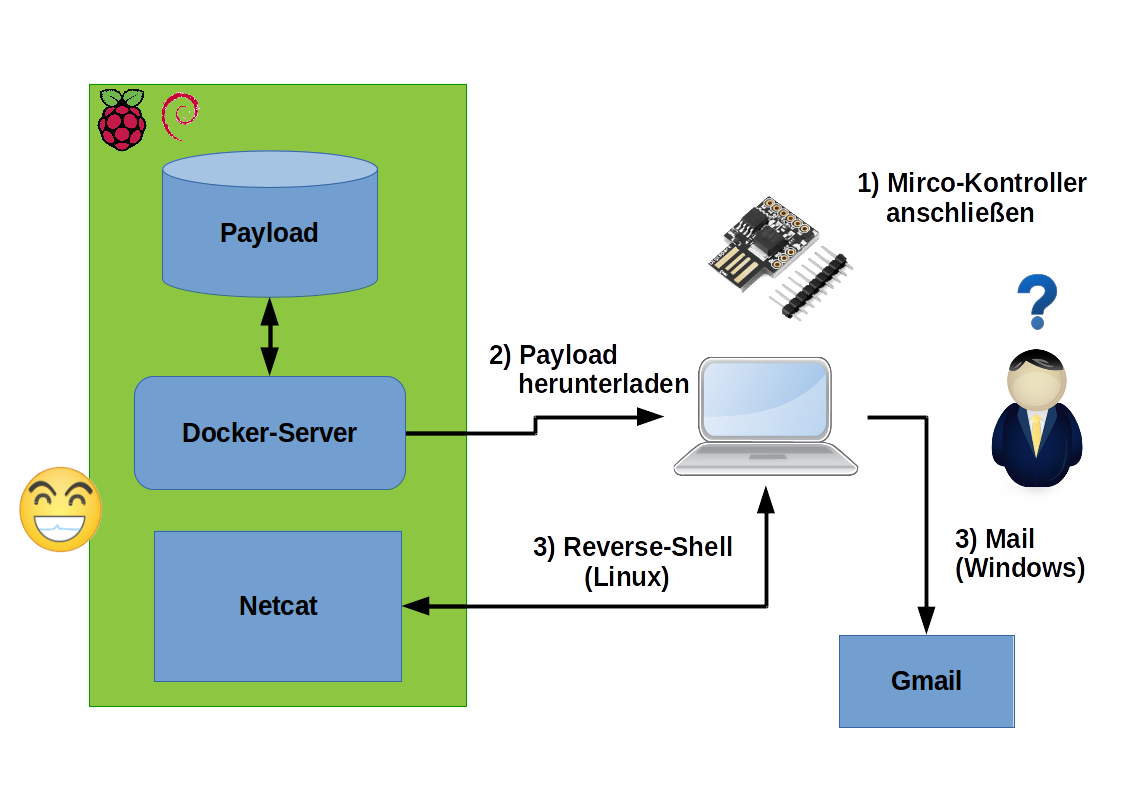
\includegraphics[width=\textwidth]{images/fakeusb/Keylogger_Ueberblick}
	\caption{Ablauf des Fake-USB Angriffs}
	\label{fig:fake_usb_ablauf}
\end{figure}

Wird ein Linux-Rechner angegriffen muss als erstes auf dem Raspberry Pi netcat gestartet werden. Mit netcat wird auf die noch aufzubauende Rerverse-Shell gewartet. Dafür wird folgender Befehl ausgeführt:

\begin{lstlisting}
nc -l -p 1234
\end{lstlisting}

\begin{itemize}
\item \bashCommand{-l} führt dazu, dass auf einkommende TCP-Verbindungen gehört wird
\item \bashCommand{-p} gibt den Port an, in diesem Fall 1234
\end{itemize}

Die beiden nachfolgenden Schritte sind bei Windows und Linux gleich, anschließend unterscheiden sich die Umsetzungen wieder.

\begin{enumerate}
\item[1)] Zuerst schließt man den anzugreifenden Rechner an das selbe Netz wie den Raspberry Pi. Anschließend kann der Micro-Kontroller angeschlossen werden. 

\item[2)] Nun öffnet sich ein Terminal bzw. eine Command-Shell und es wird automatisch die Payload für den nächsten Angriffsschritt von dem Docker-Server des Raspberry Pis heruntergeladen. Als nächstes wird die Payload ausgeführt. Die nachfolgenden Schritte unterscheiden sich nun wieder zwischen Windows und Linux.

\item[3)]
Linux:\\
Mit dem Ausführen der Payload wird eine Reverse-Shell zu dem Raspberry Pi aufgemacht. Nun können vom Raspberry Pi aus Befehle auf dem angegriffenen Linux-Rechner ausgeführt werden. 

\item[3)]
Windows:\\
Bei Windows bewirkt die Payload, dass eine Mail an das Gmail-Konto pentest123abc@gmail.com (Passwort: rubberducky) geschickt wird.

\end{enumerate}


\section{Gegenmaßnahmen}
Der Angriff mittels eines „Fake-USB“ ist sehr effektiv, da er einfach umzusetzen ist und man leicht getäuscht werden kann.
Wichtig ist die Aufklärung über die Gefahr zum Beispiel in Form von Schulungen. Bei USB-Sticks, die gefunden werden oder auf Messen verteilt werden, sollte man sehr vorsichtig sein und diese nicht an seinen Rechner anschließen. 














